% This is LLNCS.DEM the demonstration file of
% the LaTeX macro package from Springer-Verlag
% for Lecture Notes in Computer Science,
% version 2.4 for LaTeX2e as of 16. April 2010
\documentclass{llncs}


\usepackage{array,multirow}
\usepackage{color, colortbl}
\usepackage{makeidx}  
\usepackage{rotating}
\usepackage{graphicx}

\definecolor{col1}{rgb}{0.988,0.839,0.571}
\definecolor{col2}{rgb}{0.886,0.886,0.555}
\definecolor{col3}{rgb}{0.582,0.661,0.976}
\definecolor{white}{rgb}{1,1,1}

\graphicspath{{./Figures/OasisCor/},{./Figures/OasisRegression/},{./Figures/Ellipse/}}
\DeclareGraphicsExtensions{.pdf,.png}

\begin{document}

\title{Exploratory Population Analysis with Unbalanced Optimal Transport}
\titlerunning{Exploratory Population Analysis with Unbalanced Optimal Transport}  

\author{Samuel Gerber, Marc Niethammer, Martin Styner, Stephen Aylward}
\authorrunning{Gerber et al.} 
\institute{Kitware Inc, Carborro NC 27510, USA,\\
\email{samuel.gerber@kitware.com}
\and
University of North Carolina, Chapel Hill NC 27504, USA}


\maketitle              

% What problems are we addressing?
%  - [MRI] disentangle mass from shape changes
%  - [MRI] No segmentations needed
%  - [VESSELS] unstructured point clouds
%  - [VESSELS] background blood perfusion

% What's new?
%  - Hypothesis generation
%  - Different measure to capture changes
%  - No deformable registration
%  - No parameter tuning
%  - [MRI] Unbalanced mass transport
%  - [VESSELS] Decomposition of transport plan with respect to underlying measure


\begin{abstract}
The plethora of data from neuroimaging studies provide a rich opportunity to
discover effects and generate hypotheses through exploratory data analysis. The
pathologies in brain disease often manifest in changes in shape along with
deterioration and alteration of brain matter, i.e. changes in mass. We propose
to use unbalanced optimal transport to disentangle shape from mass changes and
localize those changes. The exploratory analysis approach generates images of
transport cost and mass changes for each subject in the population.  Using
voxelwise correlations with disease indicators on these images highlight
regions of mass or shape changes related to the disease indicator.  We
demonstrate the method on the white and gray matter segmentations from the
OASIS brain MRI data set, which includes subject ranging from healthy to mild
and moderate dementia. The results corroborate known pathology changes related
to dementia and suggest avenues for further clinical research. Additionally
regression and permutation testing on the transport cost and mass change images
improve on existing methods to predict disease measures and indicates that the
proposed method captures a larger portion of pathology induced changes.
\end{abstract}



\section{Introduction}
Neurological disease and disorder manifest in subtle and varied changes in
brain anatomy. To detect and quantify these changes is a primary goal of
morphometry based population analysis. 

Voxel-based morphometry (VBM) is a popular approach to detect anatomical
changes by comparing intensities at each voxel after registration of each
subject in the population to an atlas or template. We propose to use unbalanced
optimal transport to derive voxel based measures that decouple shape from
volume changes and mitigates issues with imperfect registration.
Instead of comparing intensities at each voxel, we derive for each subject two
new images based on averaging the unbalanced optimal transport solution to each
other subject. The first image measures and localizes changes in volume by
capturing the optimal allocation of mass such that resulting balanced optimal
transport problem has minimal cost. The second image measures and localizes
changes in shape an location by capturing the amount and distance that mass is
transported. Figure~\ref{fig:cor-ellipse} illustrates these two measures on a
toy example of a hundred half ellipses with different ellipticity and volume.
Correlating the derived measures from the unbalanced optimal transport
solutions with either ellipticity or total ellipse volume shows that the
proposed method is capable of correctly attributing changes to either variation
in shape or size. Intensity based VBM does not indicate the source of the
changes and results in weak correlation with changes in size.
\begin{figure}
\centering
\begin{tabular}{|c|}
\hline
\begin{tabular}{c||c}
\begin{tabular}{cc}

\includegraphics[width=0.1\linewidth]{ellipse0001} &

\includegraphics[width=0.1\linewidth]{ellipse0002} \\

\includegraphics[width=0.1\linewidth]{ellipse0003} &

\includegraphics[width=0.1\linewidth]{ellipse0004} \\

\includegraphics[width=0.1\linewidth]{ellipse0005} &

\includegraphics[width=0.1\linewidth]{ellipse0006} \\
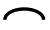
\includegraphics[width=0.1\linewidth]{ellipse0007} &
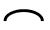
\includegraphics[width=0.1\linewidth]{ellipse0008} \\
%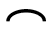
\includegraphics[width=0.1\linewidth]{ellipse0009} & 
%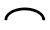
\includegraphics[width=0.1\linewidth]{ellipse0010} \\ 
\end{tabular}
        &
\begin{tabular}{l|c|c|c}
\rowcolor{col3}
Intensity&
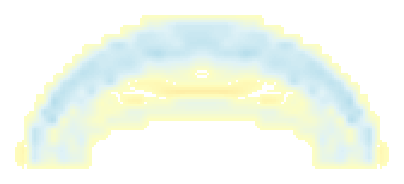
\includegraphics[width=0.18\linewidth]{cor-mass-intensity} &
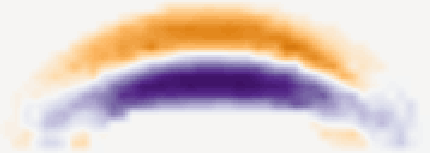
\includegraphics[width=0.18\linewidth]{cor-rx-ry-intensity} &
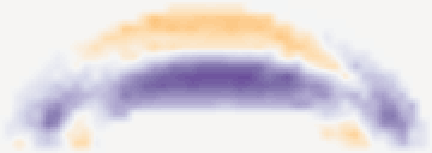
\includegraphics[width=0.18\linewidth]{cor-rx-ry-mass-intensity} \\ \hline
\rowcolor{col1}
Mass&
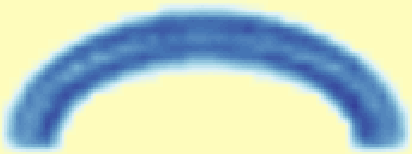
\includegraphics[width=0.18\linewidth]{cor-mass-mass} &
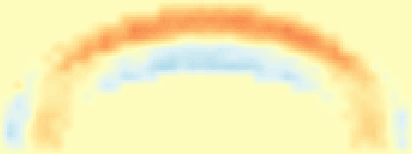
\includegraphics[width=0.18\linewidth]{cor-rx-ry-mass} &
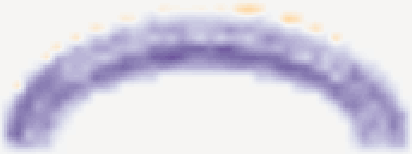
\includegraphics[width=0.18\linewidth]{cor-rx-ry-mass-mass} \\
\rowcolor{col2}
Cost&
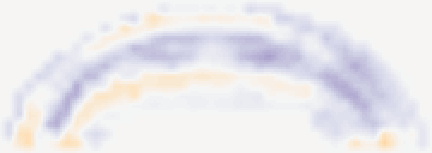
\includegraphics[width=0.18\linewidth]{cor-mass-cost} &
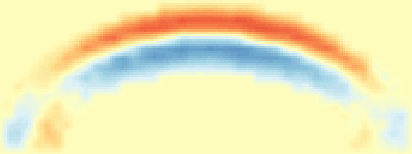
\includegraphics[width=0.18\linewidth]{cor-rx-ry-cost} &
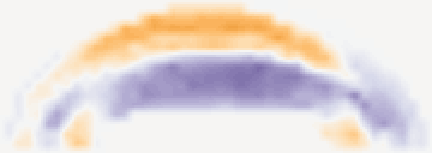
\includegraphics[width=0.18\linewidth]{cor-rx-ry-mass-cost} \\ \hline 
\rowcolor{white}
        &  Size & Ellipticity & Ellipticity + Size
\end{tabular} \\
        (a) Data Set Examples & (b) Spatial Distribution of Correlations
\end{tabular}
        \\ \hline \hline 
\begin{tabular}{c|c|c}
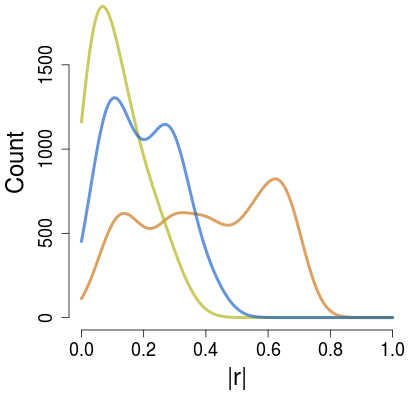
\includegraphics[width=0.3\linewidth]{hist-mass} &
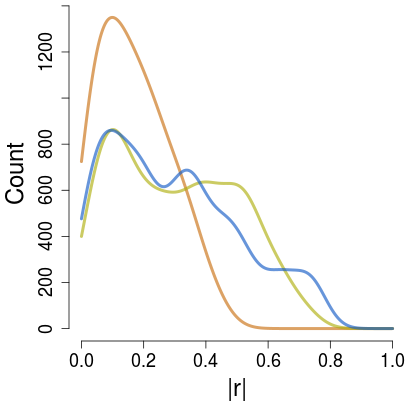
\includegraphics[width=0.3\linewidth]{hist-ellipticity} &
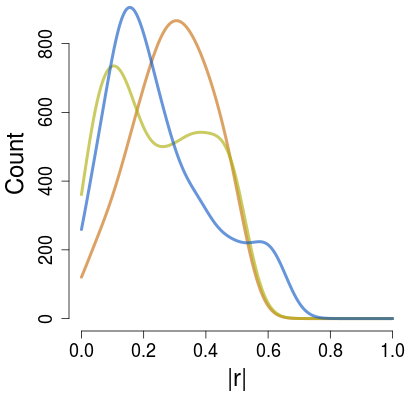
\includegraphics[width=0.3\linewidth]{hist-additive} \\ \hline 
        Size & Ellipticity & Ellipticity + Size
\end{tabular}\\
        (c) Smoothed Correlation Counts\\
        \hline
\end{tabular}
\caption{\label{fig:cor-ellipse}
Illustration of unbalanced optimal transport on a (a) toy data set of a 100
half ellipses with different minor, major radii and width.  (b) Spatial
correlations of total size (number of black pixels), ellipticity (ratio of the
minor and major radii) and sum of size and ellipticity to (top) raw pixel
intensity values, (middle) transport mass imbalances and (bottom)
transport costs. (c) Smoothed counts of Pearson's r correlation from the
spatial correlations ( colors correspond to the color of the rows in (b)). The
optimal transport approach identifies the changes in total size in the mass
imbalance with much stronger correlations than the intensity based approach.
Ellipticity is captured in both transport cost and intensity, with slightly
stronger correlations with transport cost.The shape versus mass changes in
correlations with size versus ellipticity are clearly identified in the optimal
transport based approach, while the intensity based approach alone does not
indicate the source of the correlations.  Correlation to an additive shape and
mass effect are correctly identified in both transport cost and mass imbalance,
while the intensity values alone lead to weak correlations.
}
\end{figure}

\section{Related Work}

%VBM
Voxel-based morphometry (VBM) yields spatially localized changes in brain
anatomy but has been shown to be sensitive to mis-registration and is incapable
of discovering globally occurring changes. 
%DBM
Deformation-based morphometry (DBM) takes
a more global approach by analysis of deformation fields. While DBM yields
overall measures of changes in shape, the results are sensitive to the
parametrization and regularization of the deformation field and require
delineation of regions of interest to average deformation field statistics. A
priori definition of regions defeats the purpose of automatic discovery of
relevant anatomical changes. 
%Manifold model
The manifold model approach extends DBM to allow for possible non-linear
relationships in the data and avoids having to select a template.
%Visualization
For both approaches visualization of relevant changes is difficult.
%OT map based
In \cite{} propose an optimal transport based approach that is similar to DBM
but uses a optimal transport map parametrization to a template. The approach 
%OT voxel based, this work
The unbalanced optimal transport approach presents a mixture between VBM and
DBM based methods.  While the resulting analysis is voxelwise, the quantities
compared stem from a global optimization problem which mitigates some of the
issues of a traditional VBM and introduces a way that moves towards separating
effects due to changes in volume from effects due to changes in shape.



\section{Unbalanced Optimal Transport for Population Analysis}

\section{Application to OASIS Brain MRI}

The results on the gray matter mask show an increase in the pons area
correlated with CDR and even more so with MMSE.  A hypointense T1 signal in the
pons area has been associated central pontine myelinolysis, which is linked to
alcoholism. The pons in healthy patients typically identified as white matter,
the hypointense signal could potentially lead to a identification with gray
matter, leading to a surplus of gray matter in that area.

\begingroup
\renewcommand{\arraystretch}{0}
\setlength{\tabcolsep}{0pt}
\begin{figure}[!b]
\centering
\begin{tabular}{l|cc|cc|cc} 
\parbox[t]{4mm}{\multirow{3}{*}{\rotatebox[origin=c]{90}{Mass Imbalance}}}&
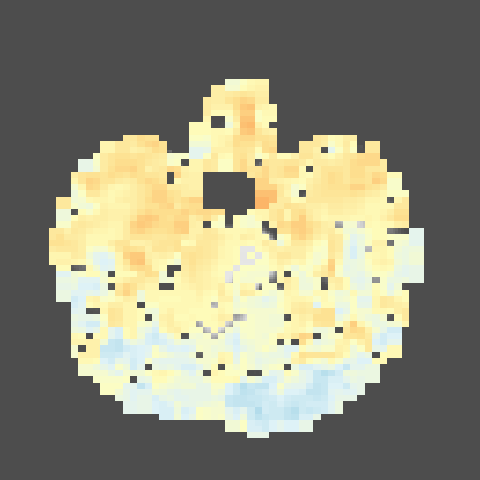
\includegraphics[width=0.16\linewidth]{cor-axial-age-mW} &
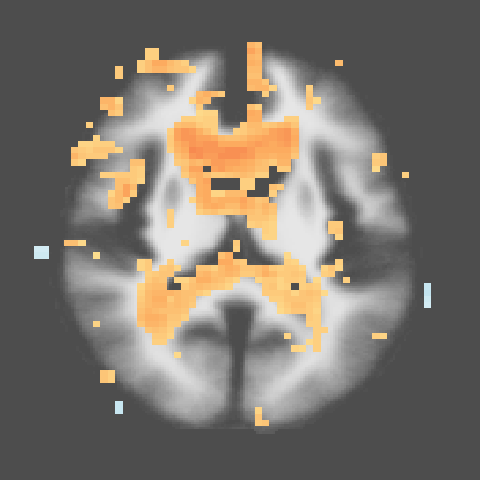
\includegraphics[width=0.16\linewidth]{cor-axial-age-t-mW} &
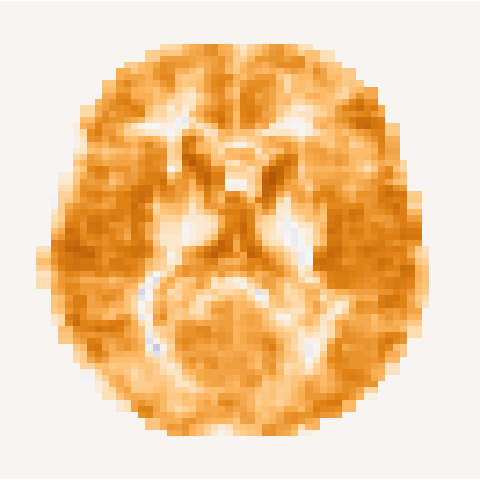
\includegraphics[width=0.16\linewidth]{cor-axial-cdr-mW} &
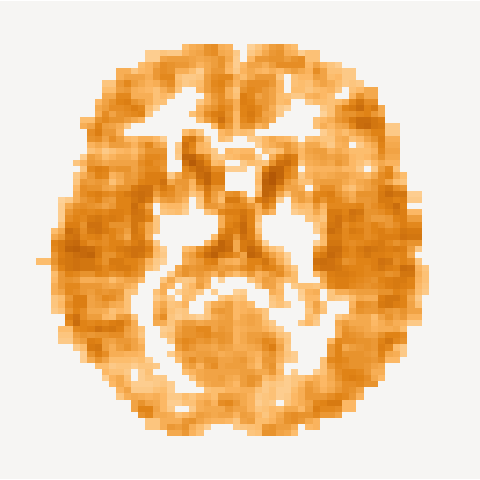
\includegraphics[width=0.16\linewidth]{cor-axial-cdr-t-mW} &
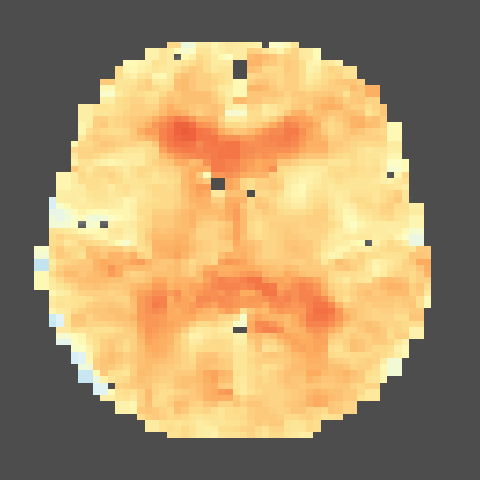
\includegraphics[width=0.16\linewidth]{cor-axial-mmse-mW} &
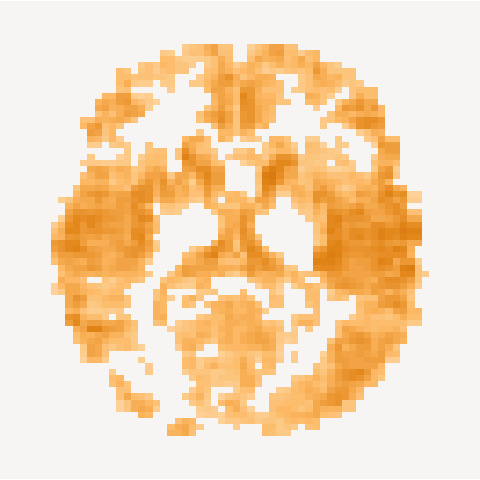
\includegraphics[width=0.16\linewidth]{cor-axial-mmse-t-mW} \\ 
%
        &
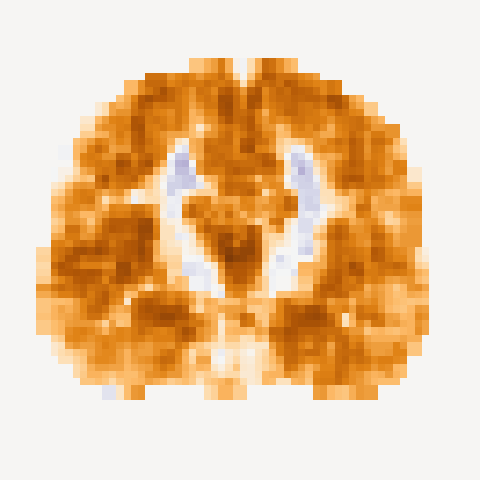
\includegraphics[width=0.16\linewidth]{cor-coronal-age-mW} &
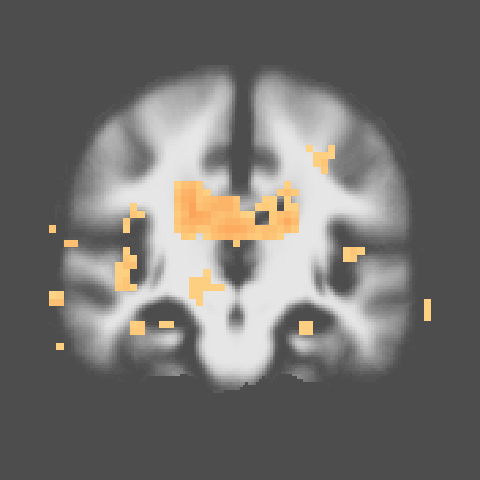
\includegraphics[width=0.16\linewidth]{cor-coronal-age-t-mW} &
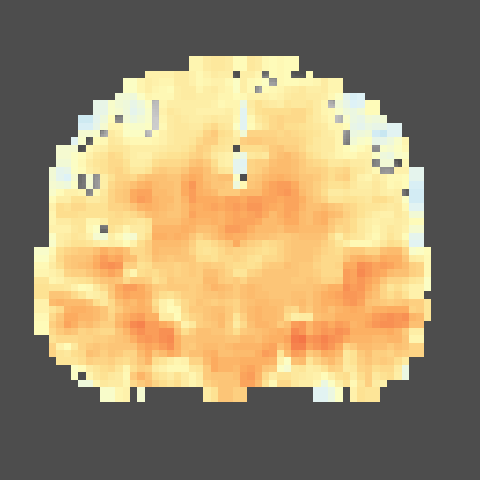
\includegraphics[width=0.16\linewidth]{cor-coronal-cdr-mW} &
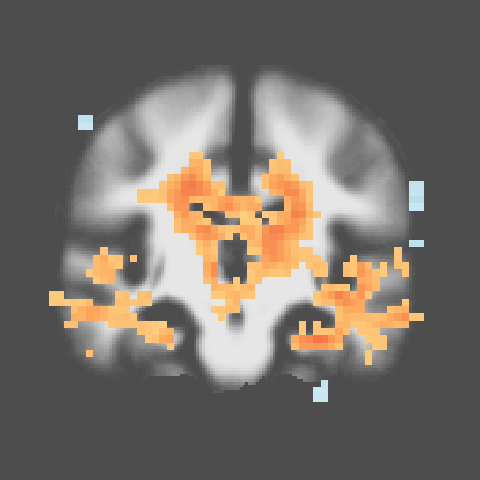
\includegraphics[width=0.16\linewidth]{cor-coronal-cdr-t-mW} &
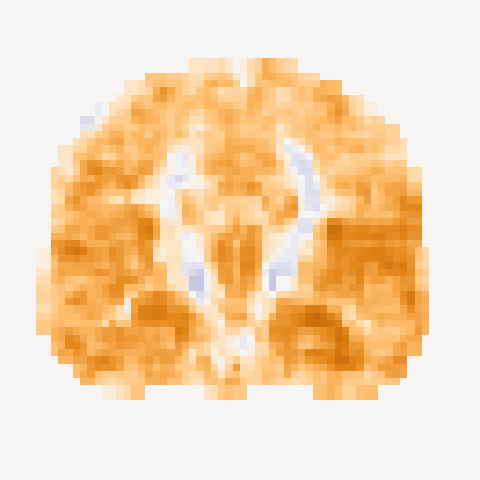
\includegraphics[width=0.16\linewidth]{cor-coronal-mmse-mW} &
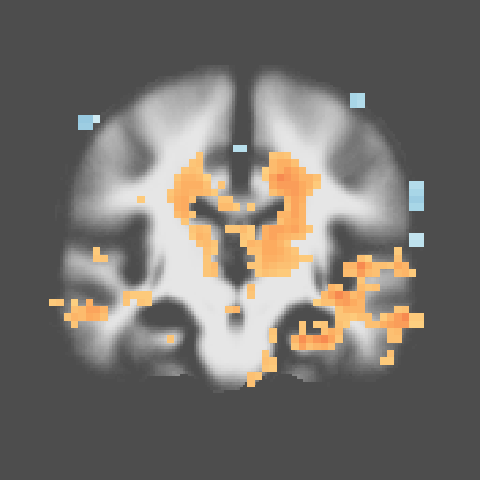
\includegraphics[width=0.16\linewidth]{cor-coronal-mmse-t-mW} \\ 
%
        &
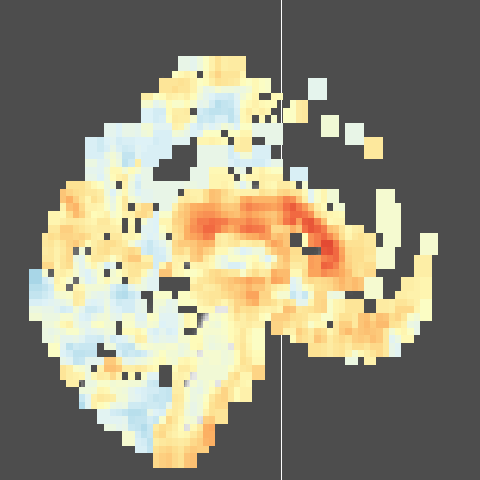
\includegraphics[width=0.16\linewidth]{cor-sagital-age-mW} &
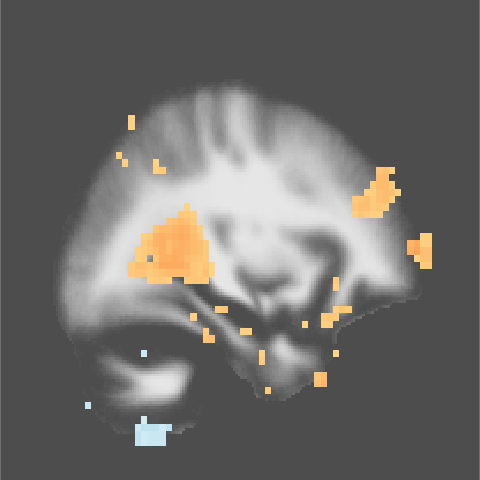
\includegraphics[width=0.16\linewidth]{cor-sagital-age-t-mW} &
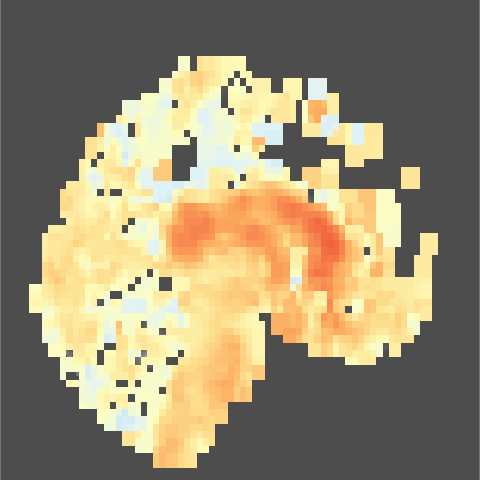
\includegraphics[width=0.16\linewidth]{cor-sagital-cdr-mW} &
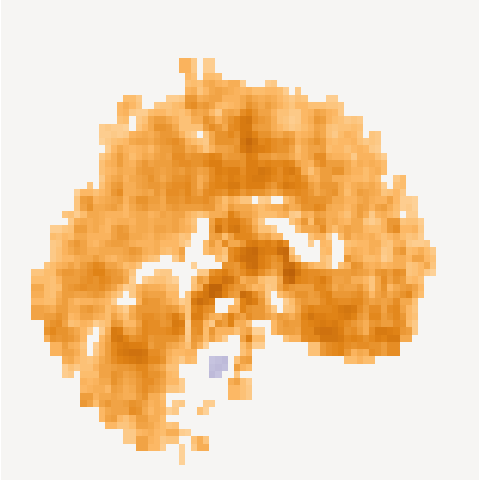
\includegraphics[width=0.16\linewidth]{cor-sagital-cdr-t-mW} &
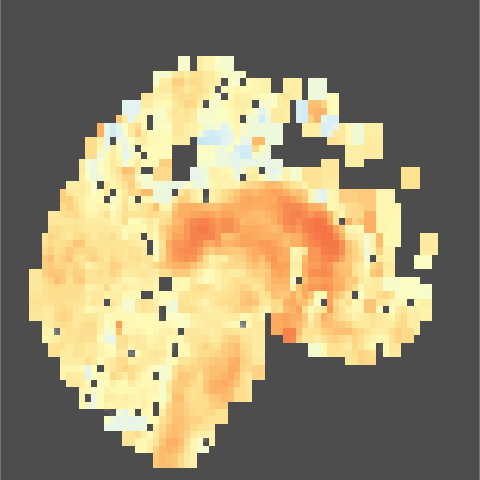
\includegraphics[width=0.16\linewidth]{cor-sagital-mmse-mW} &
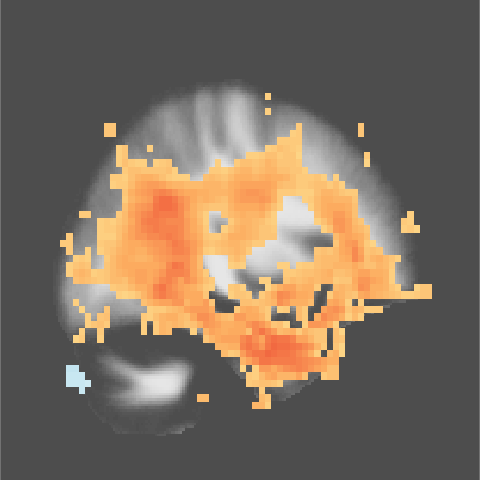
\includegraphics[width=0.16\linewidth]{cor-sagital-mmse-t-mW} \\ \hline \hline
%
\parbox[t]{2mm}{\multirow{3}{*}{\rotatebox[origin=c]{90}{Transport Cost}}}&
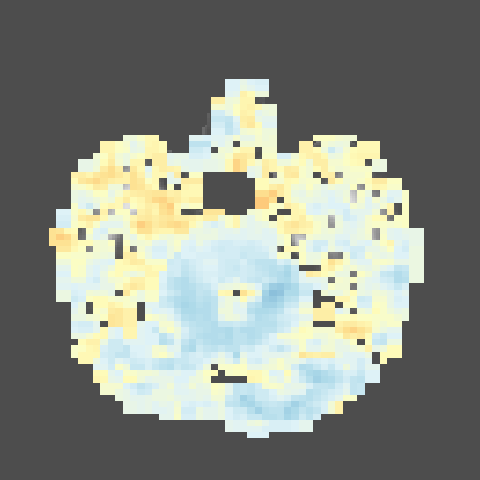
\includegraphics[width=0.16\linewidth]{cor-axial-age-tW} &
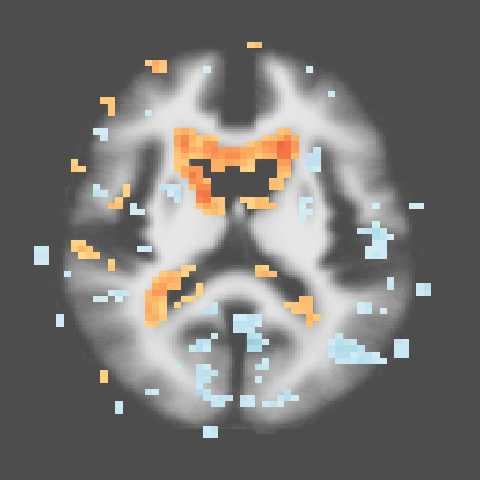
\includegraphics[width=0.16\linewidth]{cor-axial-age-t-tW} &
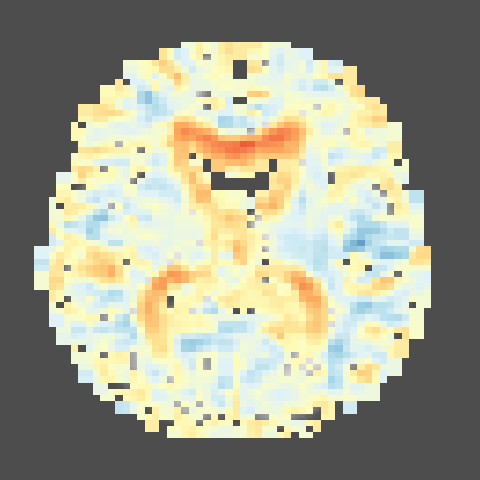
\includegraphics[width=0.16\linewidth]{cor-axial-cdr-tW} &
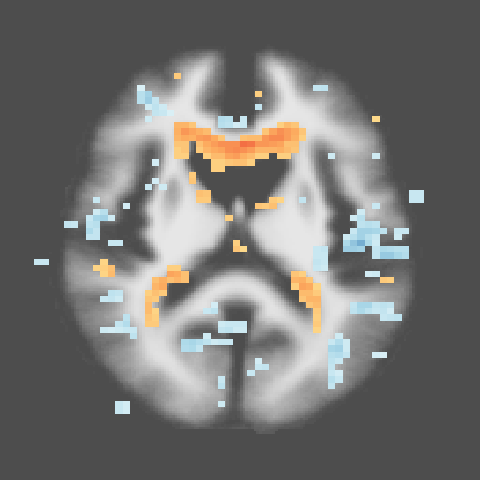
\includegraphics[width=0.16\linewidth]{cor-axial-cdr-t-tW} &
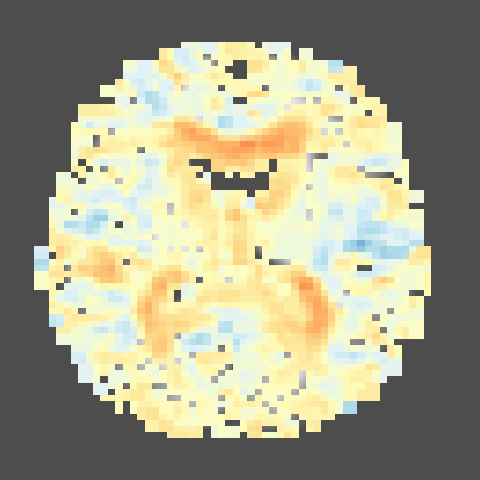
\includegraphics[width=0.16\linewidth]{cor-axial-mmse-tW} &
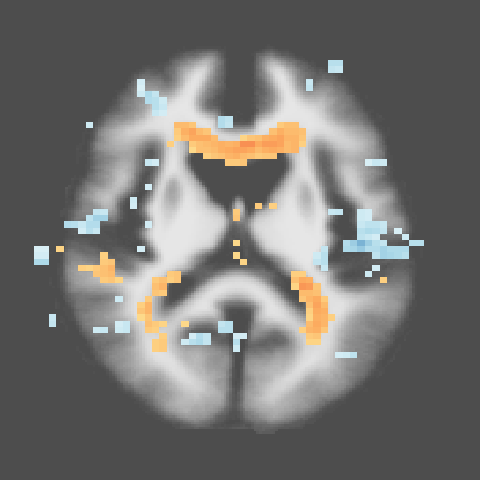
\includegraphics[width=0.16\linewidth]{cor-axial-mmse-t-tW} \\ 
%
        &
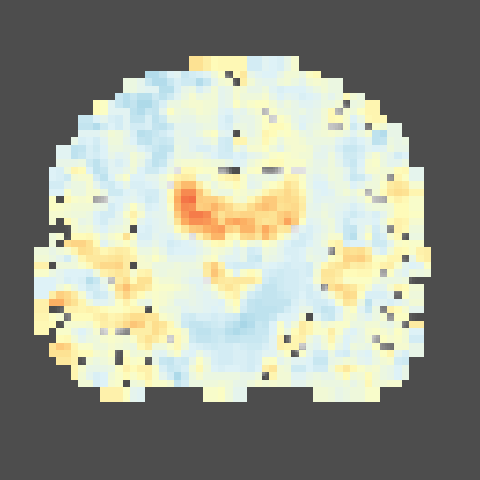
\includegraphics[width=0.16\linewidth]{cor-coronal-age-tW} &
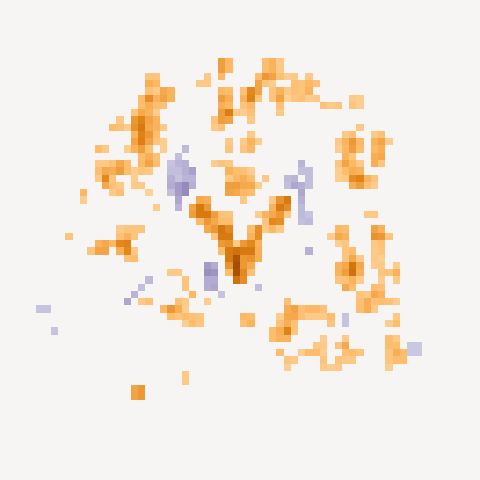
\includegraphics[width=0.16\linewidth]{cor-coronal-age-t-tW} &
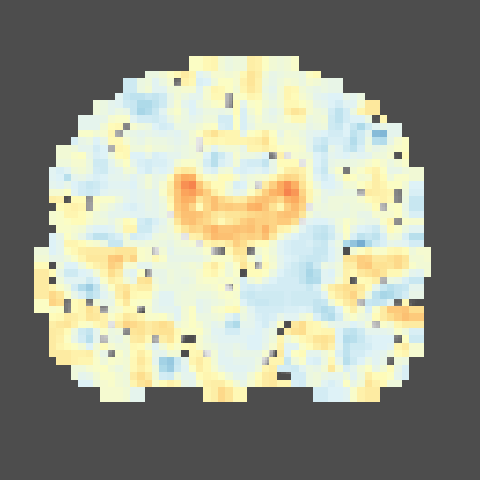
\includegraphics[width=0.16\linewidth]{cor-coronal-cdr-tW} &
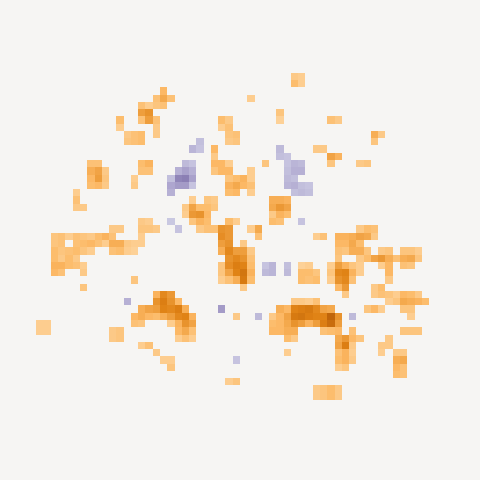
\includegraphics[width=0.16\linewidth]{cor-coronal-cdr-t-tW} &
\includegraphics[width=0.16\linewidth]{cor-coronal-mmse-tW} &
\includegraphics[width=0.16\linewidth]{cor-coronal-mmse-t-tW} \\ 
%
        &
\includegraphics[width=0.16\linewidth]{cor-sagital-age-tW} &
\includegraphics[width=0.16\linewidth]{cor-sagital-age-t-tW} &
\includegraphics[width=0.16\linewidth]{cor-sagital-cdr-tW} &
\includegraphics[width=0.16\linewidth]{cor-sagital-cdr-t-tW} &
\includegraphics[width=0.16\linewidth]{cor-sagital-mmse-tW} &
\includegraphics[width=0.16\linewidth]{cor-sagital-mmse-t-tW} \\ \hline \hline
%
& \parbox[b][4mm]{6mm}{Age} 
& \parbox[b][4mm]{6mm}{Age\textsuperscript{*}} 
& \parbox[b][4mm]{6mm}{CDR} 
& \parbox[b][4mm]{6mm}{CDR\textsuperscript{*}}
& \parbox[b][4mm]{6mm}{MMSE}
& \parbox[b][4mm]{6mm}{MMSE\textsuperscript{*}}
\end{tabular}
\caption{\label{fig:cor-oasis-white}
Correlation of age, MMSE and CDR with optimal transport mass imbalances and
optimal transport costs of white matter. The columns with a \textsuperscript{*}
only show the voxels were the correlation has a permutation tested p-value less
than 0.05  }
\end{figure}
\endgroup

\begingroup
\renewcommand{\arraystretch}{0}
\setlength{\tabcolsep}{0pt}
\begin{figure}[!b]
\centering
\begin{tabular}{l|cc|cc|cc}
\parbox[t]{4mm}{\multirow{3}{*}{\rotatebox[origin=c]{90}{Mass Imbalance}}}&
\includegraphics[width=0.16\linewidth]{cor-axial-age-mG} &
\includegraphics[width=0.16\linewidth]{cor-axial-age-t-mG} &
\includegraphics[width=0.16\linewidth]{cor-axial-cdr-mG} &
\includegraphics[width=0.16\linewidth]{cor-axial-cdr-t-mG} &
\includegraphics[width=0.16\linewidth]{cor-axial-mmse-mG} &
\includegraphics[width=0.16\linewidth]{cor-axial-mmse-t-mG} \\ 
%
        &
\includegraphics[width=0.16\linewidth]{cor-coronal-age-mG} &
\includegraphics[width=0.16\linewidth]{cor-coronal-age-t-mG} &
\includegraphics[width=0.16\linewidth]{cor-coronal-cdr-mG} &
\includegraphics[width=0.16\linewidth]{cor-coronal-cdr-t-mG} &
\includegraphics[width=0.16\linewidth]{cor-coronal-mmse-mG} &
\includegraphics[width=0.16\linewidth]{cor-coronal-mmse-t-mG} \\ 
%
        &
\includegraphics[width=0.16\linewidth]{cor-sagital-age-mG} &
\includegraphics[width=0.16\linewidth]{cor-sagital-age-t-mG} &
\includegraphics[width=0.16\linewidth]{cor-sagital-cdr-mG} &
\includegraphics[width=0.16\linewidth]{cor-sagital-cdr-t-mG} &
\includegraphics[width=0.16\linewidth]{cor-sagital-mmse-mG} &
\includegraphics[width=0.16\linewidth]{cor-sagital-mmse-t-mG} \\ \hline \hline
%
\parbox[t]{2mm}{\multirow{3}{*}{\rotatebox[origin=c]{90}{Transport Cost}}}&
\includegraphics[width=0.16\linewidth]{cor-axial-age-tG} &
\includegraphics[width=0.16\linewidth]{cor-axial-age-t-tG} &
\includegraphics[width=0.16\linewidth]{cor-axial-cdr-tG} &
\includegraphics[width=0.16\linewidth]{cor-axial-cdr-t-tG} &
\includegraphics[width=0.16\linewidth]{cor-axial-mmse-tG} &
\includegraphics[width=0.16\linewidth]{cor-axial-mmse-t-tG} \\ 
%
        &
\includegraphics[width=0.16\linewidth]{cor-coronal-age-tG} &
\includegraphics[width=0.16\linewidth]{cor-coronal-age-t-tG} &
\includegraphics[width=0.16\linewidth]{cor-coronal-cdr-tG} &
\includegraphics[width=0.16\linewidth]{cor-coronal-cdr-t-tG} &
\includegraphics[width=0.16\linewidth]{cor-coronal-mmse-tG} &
\includegraphics[width=0.16\linewidth]{cor-coronal-mmse-t-tG} \\ 
%
        &
\includegraphics[width=0.16\linewidth]{cor-sagital-age-tG} &
\includegraphics[width=0.16\linewidth]{cor-sagital-age-t-tG} &
\includegraphics[width=0.16\linewidth]{cor-sagital-cdr-tG} &
\includegraphics[width=0.16\linewidth]{cor-sagital-cdr-t-tG} &
\includegraphics[width=0.16\linewidth]{cor-sagital-mmse-tG} &
\includegraphics[width=0.16\linewidth]{cor-sagital-mmse-t-tG} \\ \hline \hline
%%
& \parbox[b][4mm]{6mm}{Age} 
& \parbox[b][4mm]{6mm}{Age\textsuperscript{*}} 
& \parbox[b][4mm]{6mm}{CDR} 
& \parbox[b][4mm]{6mm}{CDR\textsuperscript{*}}
& \parbox[b][4mm]{6mm}{MMSE}
& \parbox[b][4mm]{6mm}{MMSE\textsuperscript{*}}
\end{tabular}
\caption{\label{fig:cor-oasis-white}
Correlation of age, MMSE and CDR with optimal transport mass imbalances and
optimal transport costs of white matter. The columns with a \textsuperscript{*}
only show the voxels were the correlation has a permutation tested p-value less
than 0.05  }
\end{figure}
\endgroup




\section{Conclusion}
Combing unbalanced optimal transport with a more globally sensitive analysis.
I.e. the resulting maps are still voxelwise and should be brought into some
correspondence or averaged.

Template free approach.

Localized mass preserving

Additional analysis methods: Clustering

\end{document}
